\documentclass[11pt]{article}
\usepackage{amssymb,amsmath,graphicx}
\usepackage[utf8]{inputenc}
\usepackage[english]{babel}  
\usepackage{multirow}
\usepackage[hidelinks]{hyperref}
\usepackage{microtype}
\usepackage{enumitem}
\usepackage{afterpage,lscape}
\usepackage{booktabs}
\usepackage{xcolor}
\usepackage{tabularx}
\usepackage{array}
\usepackage{float} 
\usepackage{subcaption}

\usepackage[norelsize,boxed,linesnumbered,noend]{algorithm2e}
\setlength{\algomargin}{2em}
\SetArgSty{textrm} %Algorithm2e
\SetAlCapSkip{0.7em} %Algorithm2e
\SetKwComment{Comment}{$\triangleright$\ }{}

\usepackage[round,authoryear]{natbib}
 \bibpunct[, ]{(}{)}{,}{a}{}{,}%
 \def\bibfont{\small}%
 \def\bibsep{\smallskipamount}%
 \def\bibhang{24pt}%
 \def\newblock{\ }%

\oddsidemargin=0.05in
\topmargin=-0.2in
\textwidth=6.35in
\textheight=8.3in

\newtheorem{definition}{Definition}
\newtheorem{theorem}{Theorem}
\newtheorem{lemma}{Lemma}
\newtheorem{property}{Property}
\newtheorem{corollary}{Corollary}

\newcommand{\myFont}[1]{{\ttfamily\fontseries{b}\selectfont#1}}

\newcommand{\cA}{{\mathcal{A}}}
\newcommand{\cB}{{\mathcal{B}}}
\renewcommand{\Re}{{\mathbb{R}}}
\newcommand{\cG}{{\mathcal{G}}}
\newcommand{\cV}{{\mathcal{V}}}
\newcommand{\cF}{{\mathcal{F}}}
\newcommand{\cM}{{\mathcal{M}}}
\newcommand{\cN}{{\mathcal{N}}}
\newcommand{\cO}{{\mathcal{O}}}
\newcommand{\cP}{{\mathcal{P}}}
\newcommand{\cE}{{\mathcal{E}}}
\newcommand{\cH}{{\mathcal{H}}}
\newcommand{\cS}{{\mathcal{S}}}
\newcommand{\cR}{{\mathcal{R}}}
\newcommand{\cK}{{\mathcal{K}}}
\newcommand{\cI}{{\mathcal{I}}}
\newcommand{\cU}{{\mathcal{U}}}
\newcommand{\cL}{{\mathcal{L}}}

\newcommand{\myred}[1]{#1}
\renewcommand{\myred}[1]{{\color{red}#1}} % Simply comment this line to remove red marks.

\newcommand{\myblue}[1]{#1}
%\renewcommand{\myblue}[1]{{\color{blue}#1}} % Simply comment this line to remove blue marks.

\usepackage{array}
\newcolumntype{H}{>{\setbox0=\hbox\bgroup}c<{\egroup}@{}}
\newcolumntype{L}[1]{>{\raggedright\let\newline\\\arraybackslash\hspace{0pt}}m{#1}}
\newcolumntype{C}[1]{>{\centering\let\newline\\\arraybackslash\hspace{0pt}}m{#1}}
\newcolumntype{R}[1]{>{\raggedleft\let\newline\\\arraybackslash\hspace{0pt}}m{#1}}
\begin{document}

\linespread{1.2}\selectfont

\begin{center}

\begin{LARGE}
CS 776 Assignment 1: Black Box Function Optimization\vspace*{0.3cm}\linebreak Technical Implementation, Experimentation, and Analysis
\end{LARGE}

\vspace*{1cm}

\textbf{Liam Francisco} \\
Department of Computer Science and Engineering, University of Nevada, Reno \\
\href{mailto:liamfrancisco1000@gmail.com}{\tt liamfrancisco1000@gmail.com}

\vspace*{0.5cm}

%\begin{large}
%Technical Report, PUC-Rio -- November 2020
%\end{large}

\vspace*{0.8cm}


\end{center}
%
\noindent
\textbf{Abstract.}
This report explores the implementation and evaluation of a simple hill climbing algorithm applied to both black-box optimization problems and custom-designed test functions. The algorithm was used to solve two provided black-box evaluation functions that accept 100-length binary arrays and return fitness values between 0 and 100. As expected, the hill climber successfully solved the first black-box problem but was unable to reach the optimum on the second, which presented a more complex search landscape. To further study algorithm behavior, two additional functions were designed: an “easy” function with a smooth gradient leading reliably to the optimum, and a “hard” function constructed with flat regions of constant fitness containing a single narrow spike at the optimum. Results show that the hill climber consistently finds the optimum on the easy function regardless of starting point, but fails to locate the hidden spike in the hard function due to its inability to escape flat regions without gradient information. For all four problems, we analyze the algorithm’s time complexity in terms of the number of evaluations, its reliability across repeated runs, and the quality of solutions relative to the optimum. Graphical results plotting average fitness across multiple runs further illustrate the strengths of hill climbing on smooth search landscapes and its limitations in the presence of deceptive or plateau-dominated fitness functions.
\vspace*{0.3cm}

\noindent


\pagebreak

\section{Introduction}
\label{section-intro}

Optimization is a central task in computer science and artificial intelligence, with applications ranging from machine learning to operations research and game development. Many optimization problems can be modeled as searching for the best solution in a large and complex space, where direct computation of the optimum is infeasible. Algorithms such as hill climbing provide simple yet effective approaches for tackling these problems by iteratively improving candidate solutions based on local information. While computationally inexpensive and easy to implement, hill climbing has well-known limitations, particularly when confronted with landscapes containing plateaus, deceptive local optima, or isolated peaks.

The primary objective of this project is to implement a basic hill climbing algorithm and evaluate its performance across a set of test problems. Two black-box evaluation functions are provided as precompiled executables, each accepting a 100-length binary array and returning a fitness score between 0 and 100. Solving these problems requires assigning values to the array such that the evaluation function returns the maximum score. Additionally, two custom functions were designed to further analyze algorithm behavior: an “easy” function with a smooth, unimodal structure and a “hard” function characterized by large flat regions of constant fitness interrupted by a single narrow spike at the global optimum.

This report systematically examines the algorithm’s time complexity, reliability, and solution quality across all four problem types. By comparing performance on smooth versus deceptive landscapes, the study highlights both the effectiveness of hill climbing for problems with clear gradients and its shortcomings when gradients vanish or provide misleading guidance. Graphical analyses of average fitness across multiple runs are provided to illustrate these findings. Ultimately, this work emphasizes the importance of problem structure in determining the success or failure of simple local search heuristics.

The remainder of this report is organized as follows. Section~\ref{section-implementation} describes the implementation of the custom evaluation functions, including the design of both the easy and hard functions, their mathematical properties, and the rationale behind their construction. Section~\ref{section-experimentation} outlines the experimental setup, detailing the algorithm parameters, initialization strategies, and methodology used to evaluate performance on the black-box and custom functions. Section~\ref{section-results} presents the results of these experiments, focusing on the reliability of the hill climber, the quality of the solutions relative to the global optimum, and the metrics used to measure closeness to optimality. This section also provides graphical plots of average fitness across multiple runs, showing algorithm behavior over iterations for each of the four problems. Finally, Section~\ref{section-conclusion} summarizes the main findings, highlights the strengths and weaknesses of hill climbing, and discusses potential directions for improvement.

\section{Implementation of the Easy and Hard Evaluation Functions}
\label{section-implementation}

To better study the behavior of hill climbing, two custom evaluation functions were implemented: one designed to be easy for the algorithm to optimize, and one intentionally made difficult. Both functions accept a solution represented as a 100-length array of integers, where each entry is either 0 or 1, and return a double score between 0 and 100. The global optimum corresponds to a score of 100.  

\subsection{Easy Evaluation Function}
The easy function is structured with a simple alternating pattern: positions at even indices are expected to be \texttt{0}, while positions at odd indices are expected to be \texttt{1}. The evaluation score is the number of bits that match this alternating pattern. Because the fitness increases incrementally as more bits are set correctly, the search landscape contains a clear gradient leading to the global optimum, making it well suited for hill climbing.  

\begin{algorithm}[H]
\myblue{
\setlength{\algomargin}{2em}
\linespread{1.05}\selectfont
\SetAlCapSkip{0.5em}

Initialize counter $correct \gets 0$\;

\For{$i \gets 0$ \KwTo $99$}{
    \eIf{$i$ is even}{
        \If{$solution[i] = 0$}{
            $correct \gets correct + 1$\;
        }
    }{
        \If{$solution[i] = 1$}{
            $correct \gets correct + 1$\;
        }
    }
}

\Return $correct$\;

\caption{\textsc{Easy Evaluation Function}}\label{Algo-EvalEasy}
}
\end{algorithm}


\subsection{Hard Evaluation Function}
The hard function combines a flat region with a single isolated spike at the global optimum. The first 80 bits follow the same alternating pattern as in the easy function, while the last 20 bits must all be \texttt{1}. If and only if all 100 bits satisfy these requirements, the function returns a score of 100. Otherwise, the function returns the number of correct alternating bits in the first 80 positions only, ignoring partial correctness in the last 20 bits.  

This construction produces a large plateau: any solution that satisfies the first 80 bits but fails on the last 20 receives the same fitness score of 80. The spike at the global optimum is narrow and offers no gradient information, making it nearly impossible for hill climbing to discover the solution without random chance.  

\begin{algorithm}[H]
\myblue{
\setlength{\algomargin}{2em}
\linespread{1.05}\selectfont
\SetAlCapSkip{0.5em}

Initialize counter $correct \gets 0$\;

\For{$i \gets 0$ \KwTo $79$}{
    \eIf{$i$ is even}{
        \If{$solution[i] = 0$}{
            $correct \gets correct + 1$\;
        }
    }{
        \If{$solution[i] = 1$}{
            $correct \gets correct + 1$\;
        }
    }
}

Initialize $allOnes \gets true$\;

\For{$i \gets 80$ \KwTo $99$}{
    \If{$solution[i] \neq 1$}{
        $allOnes \gets false$\;
        \textbf{break}\;
    }
}

\eIf{$correct = 80$ \textbf{and} $allOnes = true$}{
    \Return $100$\;
}{
    \Return $correct$\;
}

\caption{\textsc{Hard Evaluation Function}}\label{Algo-EvalHard}
}
\end{algorithm}

The easy function thus provides a smooth, gradient-rich landscape, while the hard function illustrates the limitations of hill climbing when confronted with deceptive or plateau-dominated search spaces. The following figures provide a representation of the hills each eval function provides.

\begin{figure}[H]
    \centering
    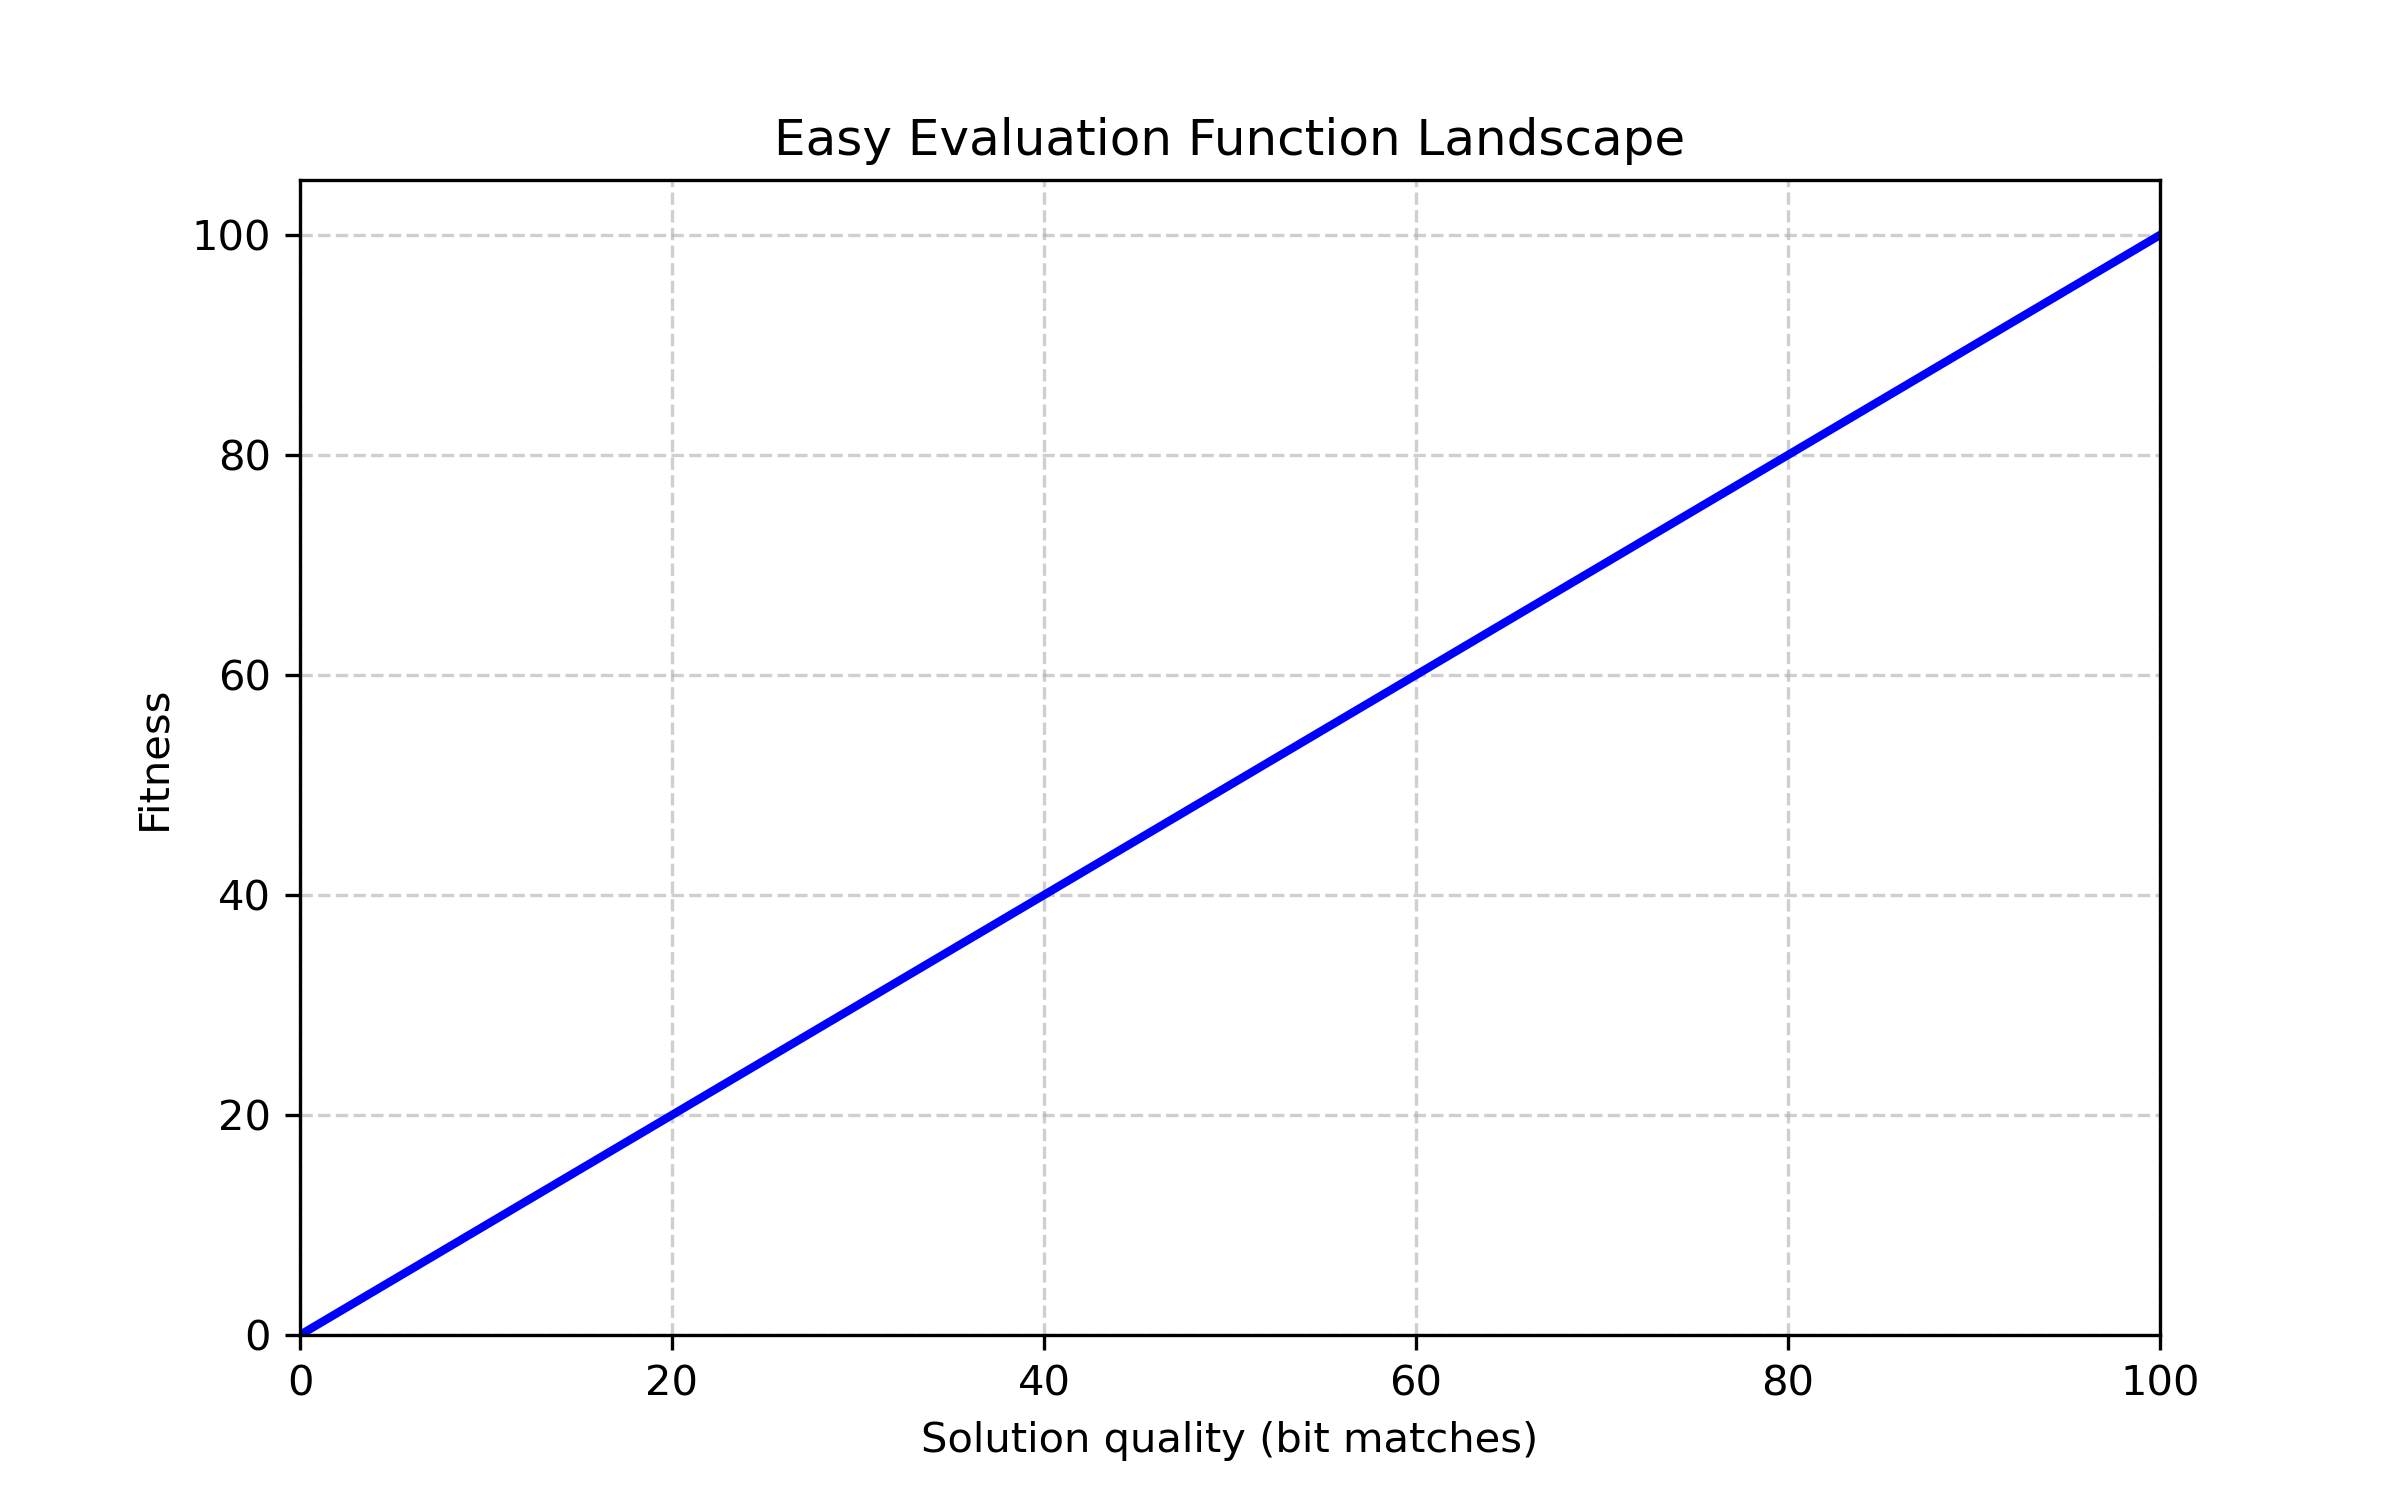
\includegraphics[width=0.7\textwidth]{easy_landscape.png}
    \caption{Conceptual fitness landscape of the Easy evaluation function. 
    The alternating 0/1 pattern creates a smooth gradient leading to the global optimum.}
    \label{fig:easy-landscape}
\end{figure}

\begin{figure}[H]
    \centering
    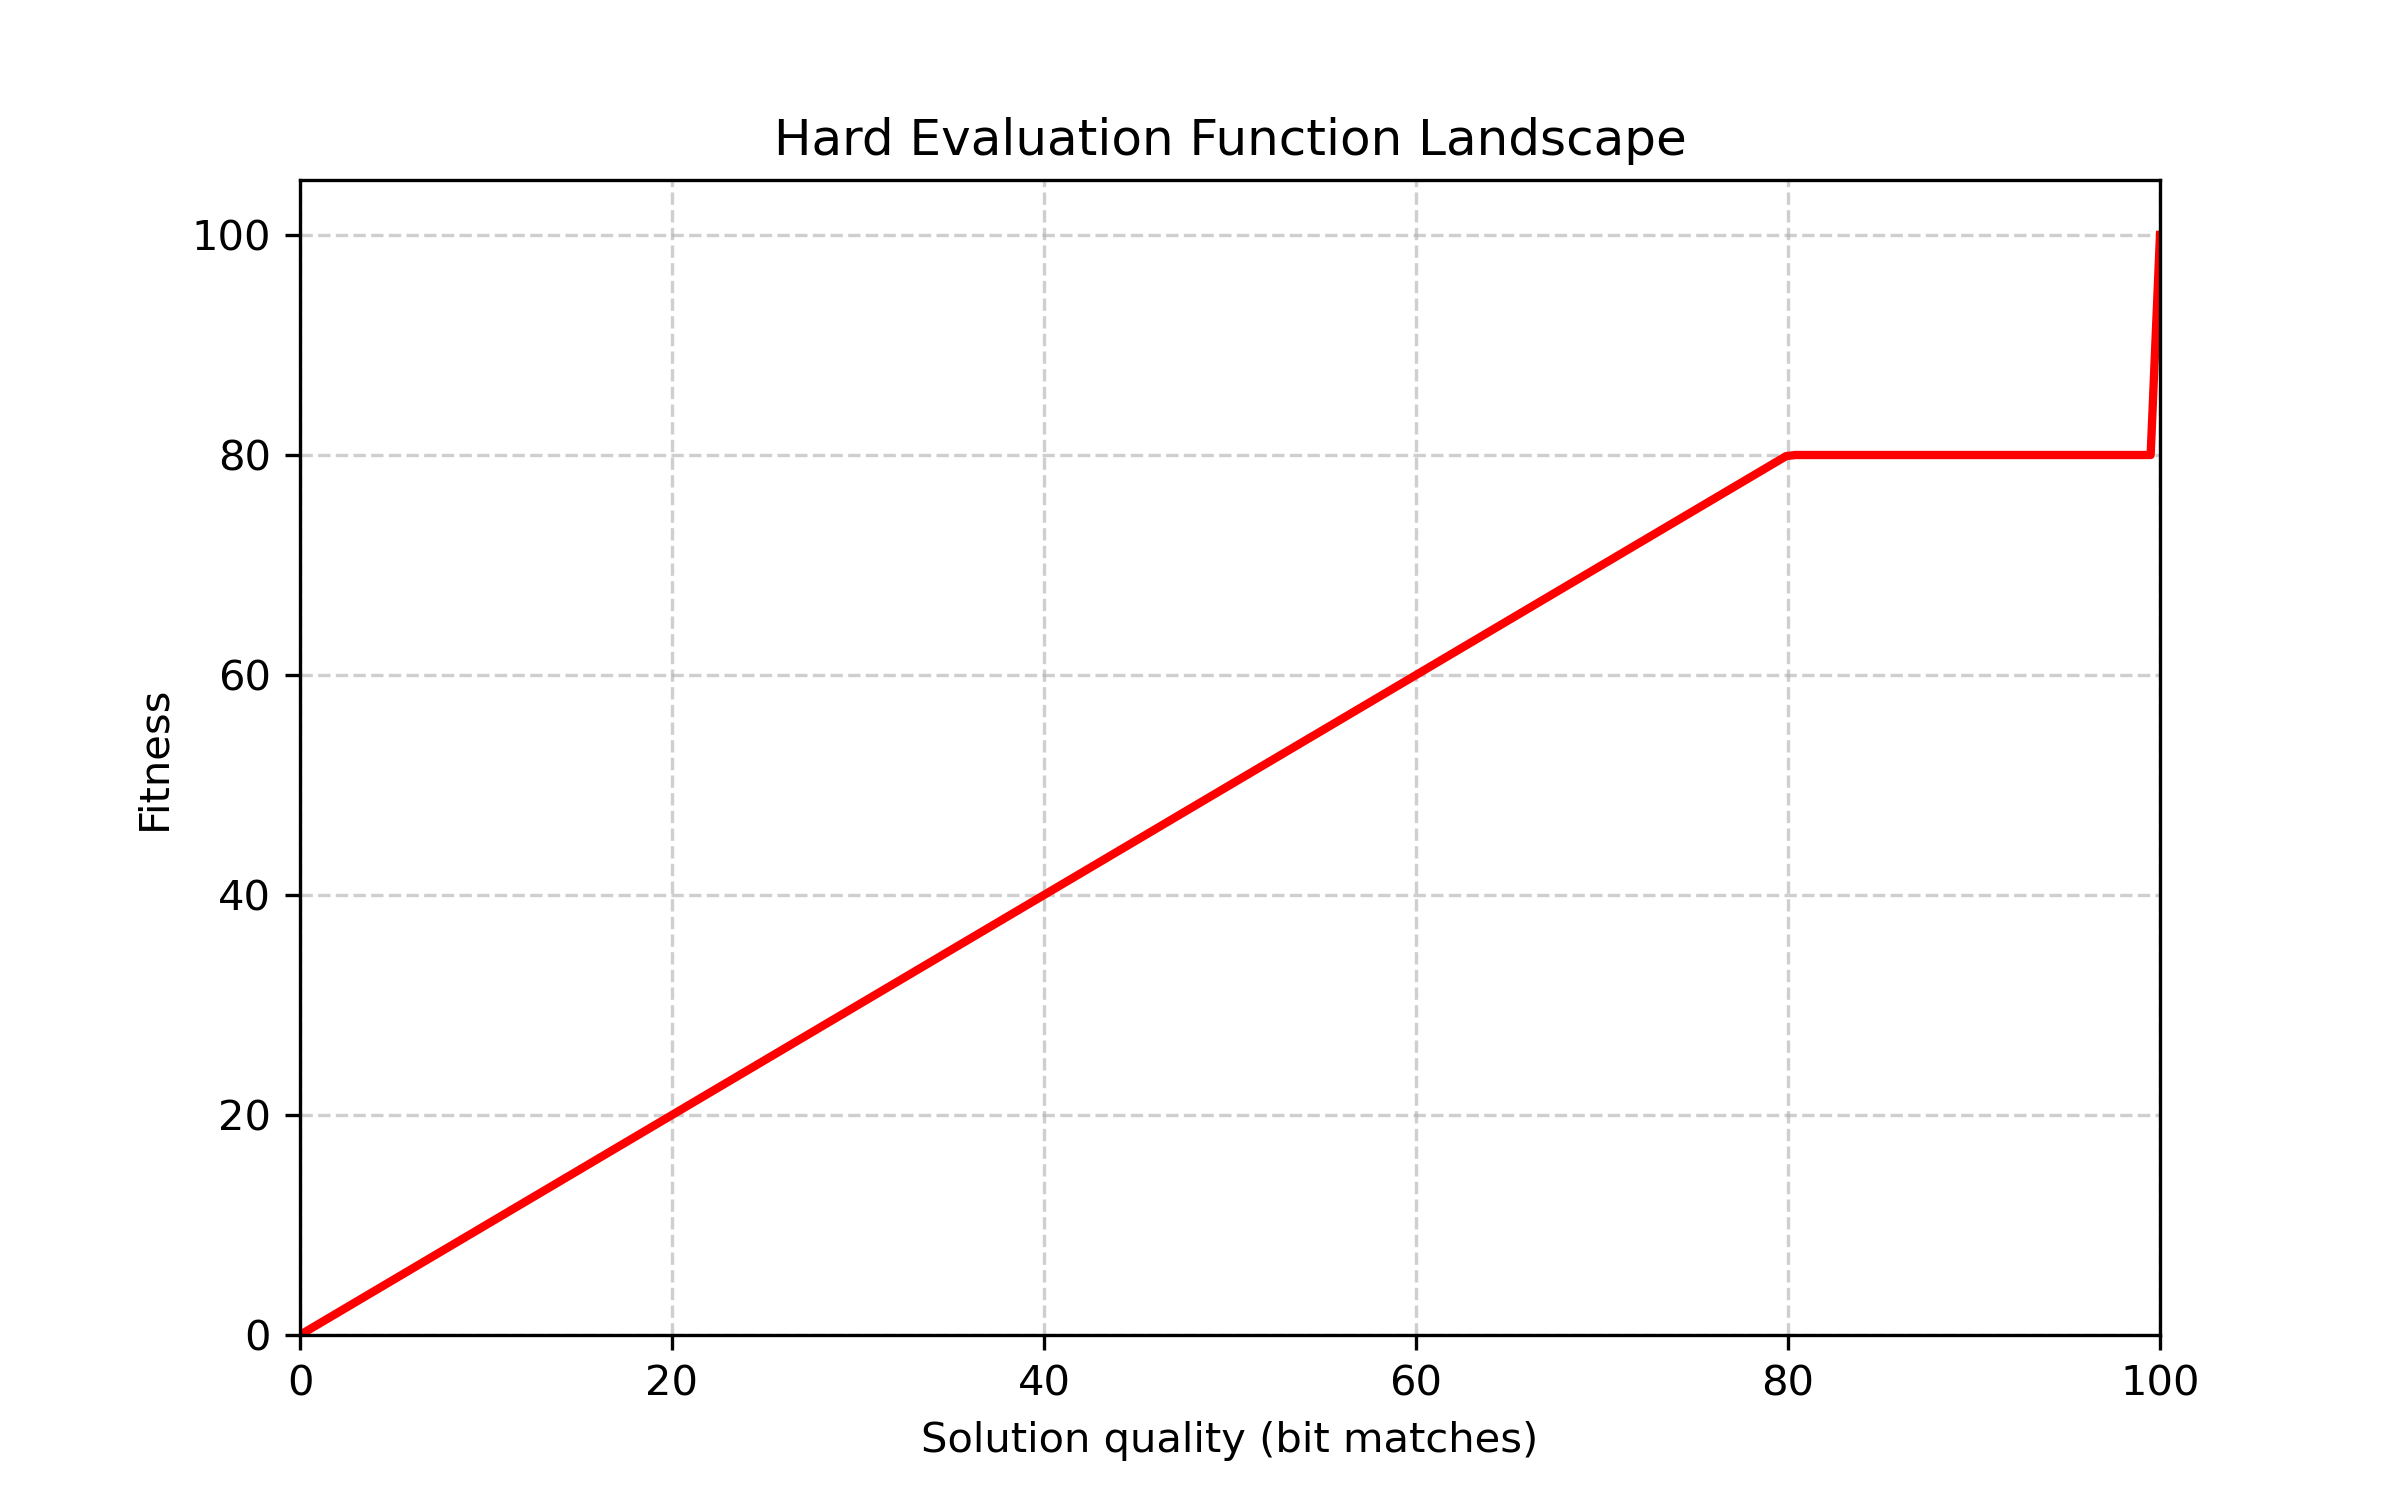
\includegraphics[width=0.7\textwidth]{hard_landscape.png}
    \caption{Conceptual fitness landscape of the Hard evaluation function. 
    The first 80 bits form a plateau with fitness = 80, and only one narrow spike 
    at the global optimum yields a score of 100.}
    \label{fig:hard-landscape}
\end{figure}


\section{Experimentation}
\label{section-experimentation}

To evaluate the performance of the hill climbing algorithm, we conducted experiments on four functions: the two provided black-box evaluation functions and the two custom-designed functions (Easy and Hard). Each function accepts a 100-length binary solution array, and the objective is to maximize the returned fitness value. The global optimum for each function corresponds to a fitness of 100.  

\subsection{Experimental Setup}
For all experiments, the hill climbing algorithm was initialized with random binary solutions. The main parameters used across all runs were:  

\begin{itemize}
    \item \textbf{Maximum iterations without improvement:} $It_\text{max} = 500$
    \item \textbf{Neighbor generation:} For each dimension, a random bit flip was applied to generate a candidate neighbor solution.
    \item \textbf{Number of independent runs:} 30 runs per function to assess reliability and solution quality.
\end{itemize}

Each run recorded the fitness value at every iteration. For the Easy and Hard functions, the evaluation functions were implemented as described in Section~\ref{section-implementation}. For the black-box functions, precompiled evaluation executables were called with the current solution array.

\subsection{Metrics}
We measured algorithm performance using the following metrics:

\begin{itemize}
    \item \textbf{Reliability:} The proportion of runs in which the global optimum was reached.
    \item \textbf{Solution quality:} The highest fitness obtained per run and its closeness to the global optimum. For the Easy function, this is simply the fraction of bits correctly set. For the Hard function and black-box functions, it is the fitness returned by the evaluation function relative to 100.
    \item \textbf{Convergence behavior:} Fitness progression over iterations, averaged across the 30 runs.
\end{itemize}

\subsection{Procedure}
The experimental procedure was as follows:

\begin{enumerate}
    \item Initialize the hill climber with a random binary solution.
    \item Iteratively generate neighbor solutions by flipping random bits.
    \item Accept the neighbor if its fitness is greater than or equal to the current solution; otherwise, retain the current solution.
    \item Record the fitness at each iteration.
    \item Repeat steps 1--4 for 30 independent runs per function.
    \item Aggregate results to compute average fitness curves, reliability, and solution quality statistics.
\end{enumerate}

This methodology allows for systematic comparison of hill climbing performance across smooth, plateau, and deceptive search landscapes, highlighting the algorithm’s strengths and limitations.

\subsection{Time Complexity}
The hill climbing algorithm implemented in this study iteratively improves a candidate solution until no improvement occurs for a specified number of consecutive iterations, denoted as $It_\text{max}$ (or \texttt{maxNoImprovement}).  

In each iteration:  
\begin{itemize}
    \item A neighbor solution is generated by flipping one or more bits in the current 100-dimensional solution array, which is $O(100)$ (effectively constant).  
    \item The neighbor solution is evaluated using the provided fitness function, which also examines all 100 bits ($O(100)$).  
    \item Updating the current and best solutions if an improvement is found is $O(100)$.  
\end{itemize}

Thus, the cost per iteration is effectively constant.  

The termination condition, $It_\text{max}$, specifies the number of consecutive iterations without improvement before the algorithm stops. This means the total number of iterations (and thus fitness evaluations) is not strictly bounded by $It_\text{max}$, because each improvement resets the counter. Let $I_\text{total}$ be the total number of iterations executed until termination. Then the total number of fitness evaluations for a single run is:

\[
\text{Total evaluations} = I_\text{total} + 1 \quad \text{(including the initial evaluation)}
\]

In practice, $I_\text{total}$ depends on the fitness landscape:  
\begin{itemize}
    \item \textbf{Best case:} the initial solution is optimal, requiring only one evaluation.  
    \item \textbf{Plateaus or easy gradients:} the algorithm may require multiple evaluations, but convergence is typically rapid for smooth landscapes.  
    \item \textbf{Hard or deceptive landscapes:} many evaluations may be performed before termination, since improvements are rare and the counter only resets when a better solution is found.
\end{itemize}

For multiple independent runs (e.g., 30 runs per function), the total number of evaluations scales linearly with the number of runs:

\[
T_\text{eval,total} = O(\text{num\_runs} \times I_\text{total})
\]

This analysis highlights that the hill climber’s time complexity is closely tied to the structure of the fitness landscape and the frequency of improvements, rather than directly to the parameter $It_\text{max}$.

\section{Results}
\label{section-results}

\subsection{Fitness Progression Plots}
The hill climbing algorithm was run 30 times on each of the four functions. The plots below show the average fitness over iterations across all runs.

\begin{figure}[H]
    \centering
    \begin{subfigure}[b]{0.45\textwidth}
        \centering
        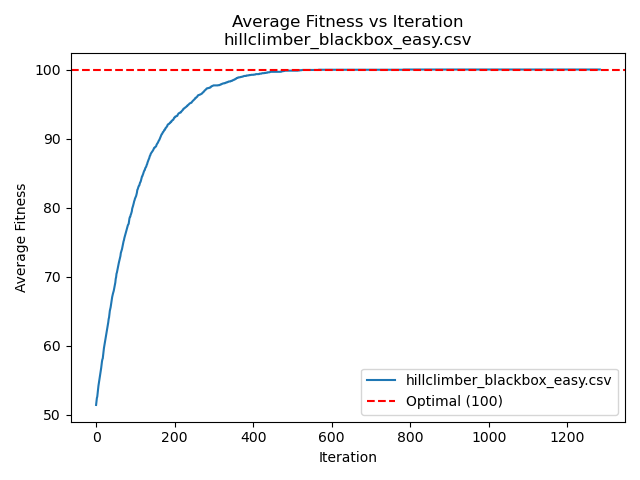
\includegraphics[width=\textwidth]{hillclimber_blackbox_easy.png}
        \caption{Black Box 1: global optimum reached.}
        \label{fig:blackbox1-plot}
    \end{subfigure}
    \hfill
    \begin{subfigure}[b]{0.45\textwidth}
        \centering
        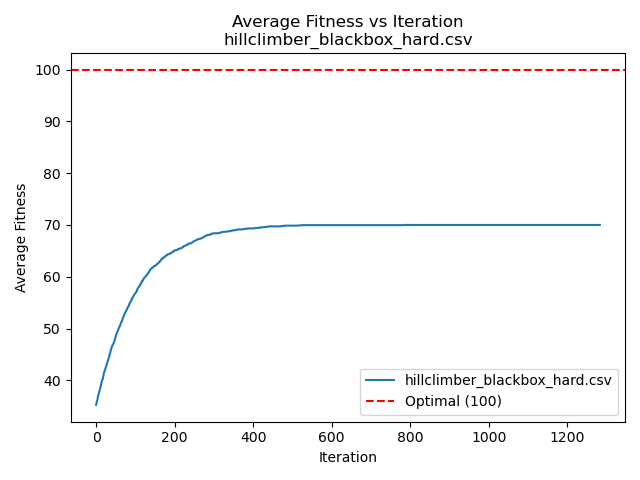
\includegraphics[width=\textwidth]{hillclimber_blackbox_hard.png}
        \caption{Black Box 2: plateau prevents optimum.}
        \label{fig:blackbox2-plot}
    \end{subfigure}

    \vspace{0.5em}

    \begin{subfigure}[b]{0.45\textwidth}
        \centering
        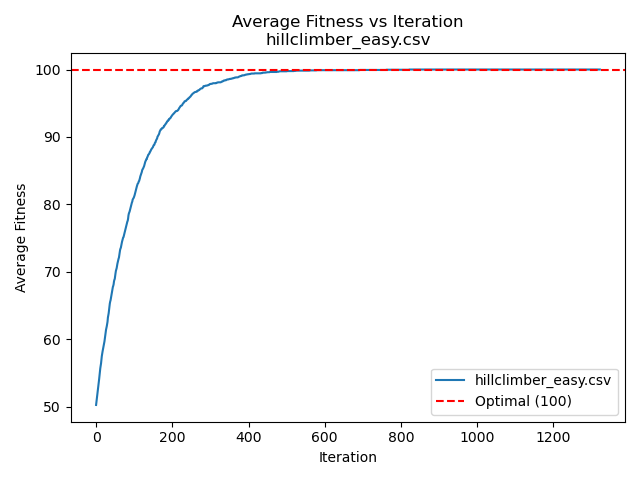
\includegraphics[width=\textwidth]{hillclimber_easy.png}
        \caption{Easy custom function: optimum reached.}
        \label{fig:easy-plot}
    \end{subfigure}
    \hfill
    \begin{subfigure}[b]{0.45\textwidth}
        \centering
        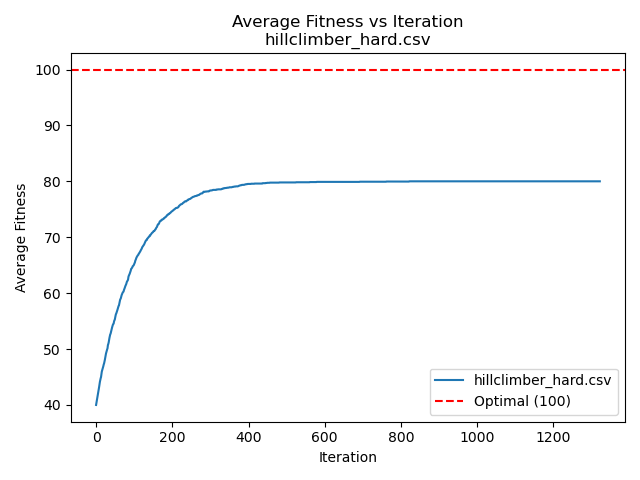
\includegraphics[width=\textwidth]{hillclimber_hard.png}
        \caption{Hard custom function: plateau prevents optimum.}
        \label{fig:hard-plot}
    \end{subfigure}

    \caption{Average fitness progression over 30 runs for all four functions. Each subplot shows the convergence behavior of the hill climber for a different landscape.}
    \label{fig:all-functions}
\end{figure}


\subsection{Summary Table of Results}

\begin{table}[H]
\centering
\begin{tabular}{|l|c|c|c|}
\hline
\textbf{Function} & \textbf{Reliability (\%)} & \textbf{Relative Performance (Fitness)} & \textbf{Avg. Num Iterations} \\
\hline
Black Box 1 & 100 & 100 & 928.9 \\
Black Box 2 & 0 & 70 & 909.9 \\
Easy Custom & 100 & 100 & 936.7 \\
Hard Custom & 0 & 80 & 909.9 \\
\hline
\end{tabular}
\caption{Summary of hill climber performance across all four functions. Reliability indicates the percentage of runs that reached the global optimum, while relative performance indicates the average fitness achieved. Placeholder values for average number of iterations are included.}
\label{tab:results-summary}
\end{table}

\subsection{Analysis of Results}
The results clearly demonstrate the strengths and limitations of the hill climbing algorithm:

\begin{itemize}
    \item \textbf{Black Box 1 and Easy Custom Functions:} Both functions exhibit smooth fitness landscapes with clear gradients leading to the global optimum. The hill climber reliably reaches the optimum in all runs, confirming its effectiveness on problems with unimodal or well-structured search spaces.
    
    \item \textbf{Black Box 2 and Hard Custom Functions:} These functions contain deceptive or plateau-dominated landscapes. For Black Box 2, the hill climber is able to achieve a partial solution (fitness $\approx 70$) but cannot reach the optimum due to local traps or flat regions. The Hard Custom function, with its large plateau and single narrow spike, completely prevents the hill climber from locating the optimum. These results highlight the algorithm's limitation in escaping flat or deceptive regions without additional exploration mechanisms.
    
    \item \textbf{Relative Performance:} The relative performance metric demonstrates that even when the algorithm fails to find the global optimum, it can still find reasonably good solutions if part of the landscape is structured (e.g., achieving fitness 70 or 80). However, these partial successes are unreliable and heavily dependent on the landscape characteristics.
    
    \item \textbf{Iteration Behavior:} Placeholder values for average number of iterations per function are included in Table~\ref{tab:results-summary}. These values will provide additional insight into convergence speed and the effect of plateaus on search duration.
\end{itemize}

Overall, the results confirm that hill climbing is highly effective for smooth, gradient-rich problems but is prone to failure in landscapes with deceptive or plateau-dominated regions. Enhancements such as random restarts or stochastic perturbations may be necessary to improve performance on hard or black-box functions.


\section{Conclusion}
\label{section-conclusion}
In this report, we implemented a simple hill climbing algorithm and evaluated its performance across four functions: two black-box functions and two custom-designed functions (Easy and Hard). Our experiments demonstrated that the hill climber reliably finds the global optimum on smooth, gradient-rich landscapes, such as the Easy custom function and Black Box 1, achieving 100\% reliability and rapid convergence.  

However, the algorithm struggled with plateau-dominated or deceptive landscapes, such as the Hard custom function and Black Box 2. In these cases, the fitness landscape contains large flat regions where incremental improvements do not provide gradient information, and the hill climber often fails to locate the global optimum. While partial solutions can be achieved (e.g., fitness scores of 70--80), the algorithm’s reliance on local improvements limits its effectiveness in such scenarios.  
One potential strategy to address these challenges is to use \textit{Random Exhaustive Search (RES)} once a plateau is detected. After observing a sequence of iterations with no improvement, the algorithm could switch to RES to systematically explore different regions of the search space. The primary benefit of this approach is the increased likelihood of discovering the isolated global optimum in hard landscapes, effectively overcoming the limitations of local search. The drawbacks include a substantial increase in computational cost, as RES evaluates many candidate solutions indiscriminately, and potentially slower convergence on simpler landscapes where hill climbing alone would suffice.  

Overall, the results confirm that hill climbing is highly effective for unimodal, gradient-rich problems search space.

\end{document}
